\section{Fondamenta degli Algoritmi Quantistici}
In questa sezione viene descritto quali sono e come vengono eseguite
le computazioni su un computer quantistico. Inizialmente vengono analizzate
le differenze che si hanno quando ci si confronta con un modello di computazione classico
e, nello specifico, verranno elencati algoritmi quantistici che offrono
vantaggi rispetto ad una computazione classica.
\subsection{Computazione classica vs Computazione quantistica}
Uno dei primi vantaggi che una computazione quantistica può offrire
è sicuramente quello del \textbf{tempo}; infatti, per alcuni problemi, sono state proposte
nuove soluzione che hanno dimostrato un incremento esponenziale del tempo di esecuzione.

Mediante l'utilizzo di porta logica di \textbf{Toffoli}, è possibile simulare circuiti 
logici classici su circuiti quantistici. La porta di \textbf{Toffoli} riesce
ad implementare un qualsiasi circuto Booleano; inoltre, la reversibilità di tale porta,
contribuisce alla simulazione dei circuiti classici su circuiti quantistici.

Ad esempio, riusciamo a simulare la porta NAND (irreversibile) con la porta di Toffoli.
La figura \ref{fig13} mostra il NAND implementato con il Toffoli gate.
\begin{figure}[h]
    \centering
    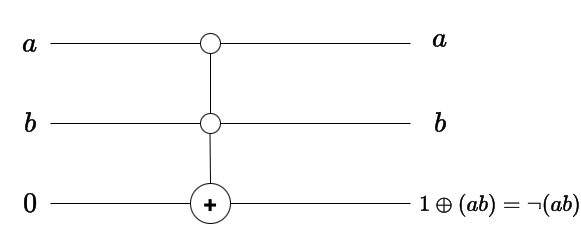
\includegraphics[width = 7cm]{./Images/toff.png}
    \caption{}
    \label{fig13}
\end{figure}

\begin{fact}{}{}
    È possibile implementare qualsiasi circuito booleano classico attraverso la porta di Toffoli.
\end{fact}

\subsection{Parallelismo Quantistico}
Data una funzione $f(x)$, definiamo (a parole semplici) il \textbf{parallelismo
quantistico} come una caratteristica del mondo quantistico che permette
la valutazione di $f(x)$ per diversi valori di $x$ simultaneamente.

Supponiamo che $f(x): \{0,1\} \rightarrow \{0,1\}$. Calcolare tale funzione
in un'ambiente quantistico necessita la definizione di un'operazione 
unitaria, solitamente chiamata $U_f$, rappresentata nella figura \ref{fig14}.
\begin{figure}[h]
    \centering
    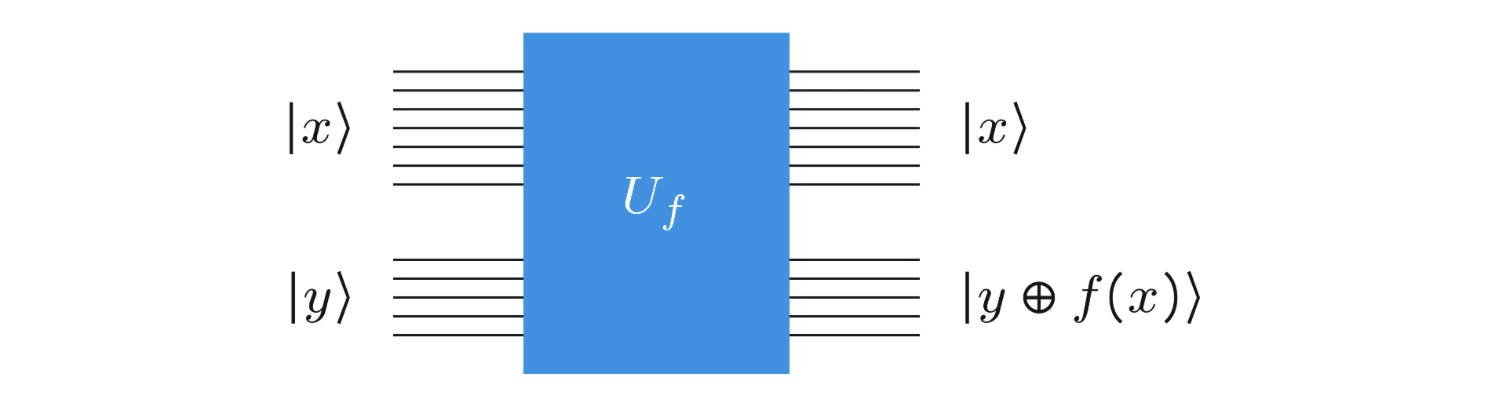
\includegraphics[width = 10cm]{./Images/uf.png}
    \caption{}
    \label{fig14}
\end{figure}
 Quindi dobbiamo considerare un computer quantistico a due qubit,
 che inizializza lo stato a $|x,y\rangle$. 
 
 Dopo l'applicazione di $U_f$, riusciamo a trasformare lo stato in $|x,y \oplus f(x)\rangle$, 
 dove $\oplus$ indica l'operazione \textit{bitwise} dello XOR. Denominiamo il primo registro come
 \textit{data} e il secondo come \textit{target}.

 \begin{oss}{}{}
    Se $y=0$, allora lo stato finale del secondo qubit è equivalente
    ad $f(x)$.
 \end{oss}

 Supponiamo ora che inizializziamo il registro \textit{data} nella superposizione
 \begin{equation*}
    |+\rangle = \frac{1}{\sqrt{2}}|0\rangle + \frac{1}{\sqrt{2}}|1\rangle
 \end{equation*}
 la quale può essere ottenuta, ad esempio, applicando la porta di Hadamard
 sullo stato base $|0\rangle$. Supponiamo anche di inizializzare il ragistro
 \textit{target} con $|0\rangle$. Quindi:
 \begin{equation*}
    \begin{array}{c}
        U_f\left(\left(\frac{1}{\sqrt{2}}|0\rangle + \frac{1}{\sqrt{2}}|1\rangle\right)\otimes |0\rangle\right) = \frac{1}{\sqrt{2}}\left(U_f \left(|0\rangle \otimes |0\rangle\right) + U_f \left(|1\rangle \otimes |0\rangle\right)\right) \\ \\
        = \frac{1}{\sqrt{2}}\left(|0\rangle \otimes |f(0)\rangle + (|1\rangle \otimes |f(1)\rangle)\right)
    \end{array}
 \end{equation*}
 Osserviamo, incredibilmente, di come ci sia bastata una singola 
 valutazione per computare la funzione su tutto il dominio della funzione ($\{0,1\}$).
 Abbiamo semplicemente sfruttato l'abilità di un qubit di stare
 in una superposizione tra stati differenti.

 Questa procedura è generalizzabile per tutte le funzioni aventi
 un numero arbitrario di bits, utilizzando un'operazione
 generale conosciuta come \textbf{trasformazione di Hadamard}, o anche
 \textbf{trasformazione di Walsh-Hadamard}. È semplicemente l'applicazione 
 di $n$ porte di Hadamard in parallelo su $n$ qubits.
 \begin{example}{}{}
    Ad esempio, per $2$ qubit inizializzati allo stato base $|0\rangle$,
    la trasformazione ci da come output:
    \begin{equation*}
        \left(\frac{|0\rangle + |1\rangle}{\sqrt{2}}\right)\left(\frac{|0\rangle + |1\rangle}{2}\right) = \frac{|00\rangle + |01\rangle +|10\rangle +|11\rangle}{\sqrt{2}}
    \end{equation*}
 \end{example}
 Nel esempio, denotiamo con $H^{\otimes 2}$ l'operazione parallela delle porte di Hadamard. Più in generale, 
 la computazione di tale trasformazione su $n$ qubit con stato di partenza a $|0\rangle$ è equivalente a
 \begin{equation*}
    \frac{1}{\sqrt{2^n}}\sum_{x \in \Sigma} |x\rangle
 \end{equation*}
ed indichiamo con $H^{\otimes n}$ tale operazione. Otteniamo una superposizione di
\textbf{$2^n$} stati usando solo \textbf{$n$} porte.

La misurazione dello stato $\frac{1}{\sqrt{2^n}}\sum_{x \in \Sigma} |x\rangle$ ci restituisce solo $f(x)$, per un singolo
valore $x$. Non ci è tanto utile, quindi è necessaria l'abilità di estrazione di informazioni
su più di un valore di $f(x)$ dalla superposizione per poter sfruttare questo parallelismo.

\subsection{Algoritmo di Deutsch}